\documentclass{standalone}% or wathever you want

% load packages
\usepackage{tikz, xcolor}
% load libraries
\usetikzlibrary{intersections,shapes.arrows,calc}

% define light and dark gray
\definecolor{lgray}{cmyk}{0,0,0,0.2}
\definecolor{dgray}{cmyk}{0,0,0,0.7}

% make some settings
\tikzset{%
    % style for the intersecting path, which
    % are nessesary for the calculation but
    % shouldn't be drawn in the final image
    ipath/.style={
%       draw,% comment this aout after construction
        red
    },
    % style for an arrow used as object
    optical arrow/.style={%
        fill=dgray,
        inner sep=3pt,
        shape=single arrow,
        minimum width=0.5cm,
        minimum height=1.5cm,
        outer sep=0pt,
        shape border rotate=90,
    },
    % style for the virtual image
    virtual optical arrow/.style={%
        fill=lgray,
        inner sep=3pt,
        shape=single arrow,
        minimum width=0.5cm,
        minimum height=1.5cm,
        outer sep=0pt,
        shape border rotate=90,
    },
    % style for the mirror
    mirror/.style={%
        line width=2pt,
    },
    % style for the axis
    optical axis/.style={%
        thin,
    },
    % style for light rays
    ray/.style={%
        thin,
        ->,
    },
    % style for imagined rays, which ar not real
    % but help by constructin the image
    imagined ray/.style={%
        ray, dgray, -,
    },
    % alias
    virtual ray/.style={imagined ray},
    % style for (focal) points
    point/.style={%
        fill=black,
        radius=0.8pt,
        inner sep=1pt,
        shape=circle,
        minimum size=2pt,
        outer sep=2pt
    },
}

% set three layers
\pgfdeclarelayer{background}
\pgfdeclarelayer{foreground}
\pgfsetlayers{background,main,foreground}
% and define shortcuts to access them
\newcommand{\bglayer}[1]{%
    \begin{pgfonlayer}{background}%
    #1%
    \end{pgfonlayer}%
}
\newcommand{\fglayer}[1]{%
    \begin{pgfonlayer}{foreground}%
    #1%
    \end{pgfonlayer}%
}

\begin{document}
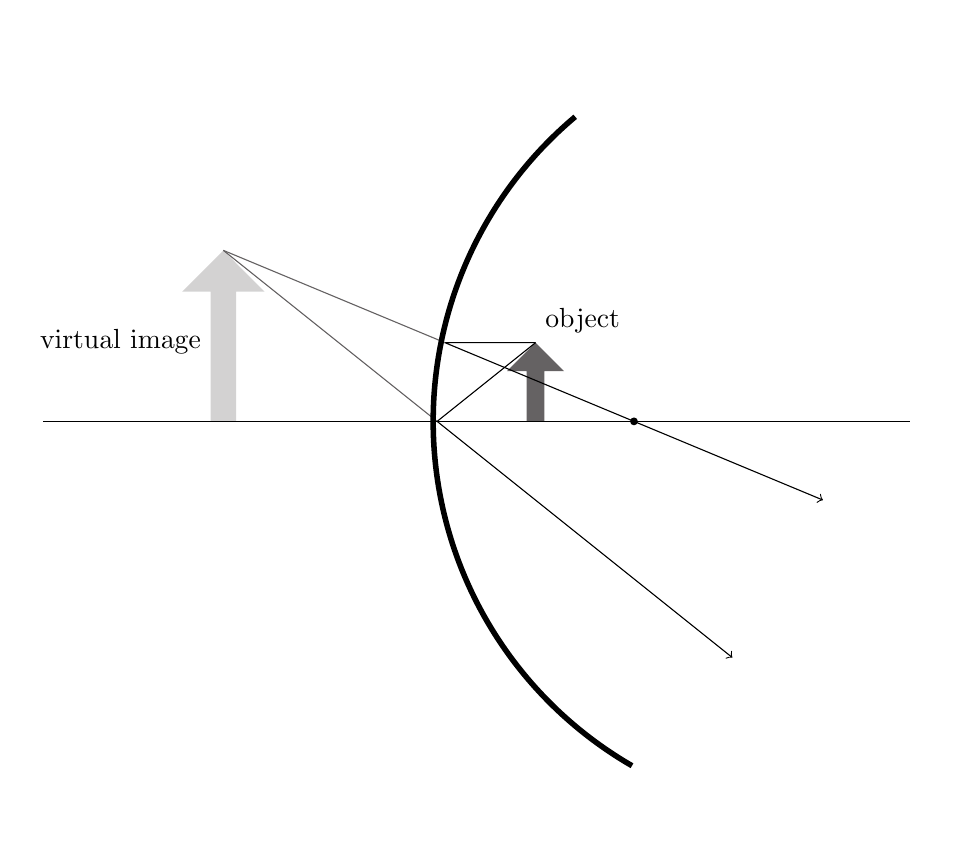
\begin{tikzpicture}
    % define the bounding box is nessesarx because the ipaths
    % make it bigger than needed
    \path [use as bounding box] (-5.2,-5) rectangle (6.2,5);
    % define variables, you may vary them a little
    %% radius
    \def\radius{5}
    \def\radiusII{5.05}
    %% focal distancs = \radius/2
    \def\focal{2.5}
    %% object size
    \def\size{1.cm}
    %% object width
    \def\owidth{1.25}
    % draw mirror
    %% the extra ipath is nessesary to get nicer rays
    \path [ipath, name path=M] (\radius,0) ++(90:\radius)
          arc (90:270:\radius);
    \fglayer{%
        \draw [mirror] (\radiusII-0.05,0) ++(130:\radiusII)
              arc (130:240:\radiusII);
    }
    % draw focal point
    \node (B) at (\focal,0) [point] {};
    % draw object
    \node (O) [optical arrow,anchor=tail, minimum height=\size] %
          at (\owidth,0) {};
    %% description
    \node [above right] at (O.tip) {object};
    % rays
    %% draw axis ray
    \draw [ray] (O.tip) -- (0,0) -- ($(0,0)!3!(\owidth,-\size)$);
    %% draw parallel ray
    \path [ipath, name path=PS] (O.tip) -- ++(-3,0);
    \draw [ray, name intersections={of=M and PS, by=M-PS}]
        (O.tip) -- (M-PS) -- ($(M-PS)!2!(B)$);
    %% caculate virtual axis ray
    \path [ipath, name path=AS-V] ($(0,0)!-4!(\owidth,-\size)$) -- (0,0);
    %% calculate virtual parallel ray
    \path [ipath, name path=PS-V] ($(M-PS)!-4!(B)$) -- (M-PS);
    %% draw virtual axis ray
    \draw [imagined ray, name intersections={of=AS-V and PS-V, by=Tip-V}]
        (Tip-V) -- (0,0);
    %% draw virtual axis ray
    \draw [imagined ray] (Tip-V) -- (M-PS);
    % draw virtual object
    \bglayer{\path let \p{1}=(Tip-V) in 
        (Tip-V) node (V) [minimum height=\size,
                          scale={\y{1}/\size*0.665},
                          virtual optical arrow,anchor=tip
                         ] {};}
    %% description
    \path (V.west) node [left] {virtual image};
    % draw optical axis
    \fglayer{\draw [optical axis] (-5,0) --++(11,0);}
\end{tikzpicture}
\end{document}
